\begin{center}
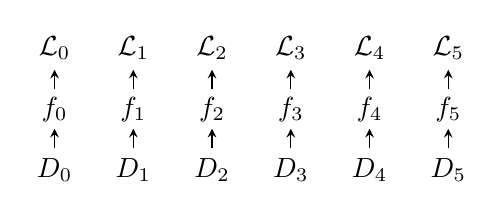
\begin{tikzpicture}
\begin{scope}[scale=0.5]
    
    
    \node (a) at (0,0) [rectangle, rounded corners] {$f_0$};
    \node (b) at (2,0) [rectangle, rounded corners] {$f_1$};
    \node (c) at (4,0) [rectangle, rounded corners] {$f_2$};
    \node (d) at (6,0) [rectangle, rounded corners] {$f_3$};
    \node (e) at (8,0) [rectangle, rounded corners] {$f_4$};
    \node (f) at (10,0) [rectangle, rounded corners] {$f_5$};
    
    \draw[-stealth] (0,0.5) -- (0, 1) node[above] {$\mathcal{L}_0$};
    \draw[-stealth] (2,0.5) -- (2, 1) node[above] {$\mathcal{L}_1$};
    \draw[-stealth] (4,0.5) -- (4, 1) node[above] {$\mathcal{L}_2$};
    \draw[-stealth] (6,0.5) -- (6, 1) node[above] {$\mathcal{L}_3$};
    \draw[-stealth] (8,0.5) -- (8, 1) node[above] {$\mathcal{L}_4$};
    \draw[-stealth] (10,0.5) -- (10, 1) node[above] {$\mathcal{L}_5$};

    
    \draw[-stealth] (0, -1) node[below] {$D_0$} -- (0, -0.5);
    \draw[-stealth] (2, -1) node[below] {$D_1$} -- (2, -0.5);
    \draw[-stealth] (4, -1) node[below] {$D_2$} -- (4, -0.5);
    \draw[-stealth] (6, -1) node[below] {$D_3$} -- (6, -0.5);
    \draw[-stealth] (8, -1) node[below] {$D_4$} -- (8, -0.5);
    \draw[-stealth] (10, -1) node[below] {$D_5$} -- (10, -0.5);
    
\end{scope}
\end{tikzpicture}
\end{center}
